\begin{blocksection}
\question What does it mean for a filter to be shift-invariant?

\begin{solution}[0.75in]
{\color{red} TBA}
\end{solution}
\end{blocksection}

%%%

\begin{blocksection}
\question Convolve the image $\mb{F}$ with filter $\mb{h}$. Assume ones beyond the boundaries. 

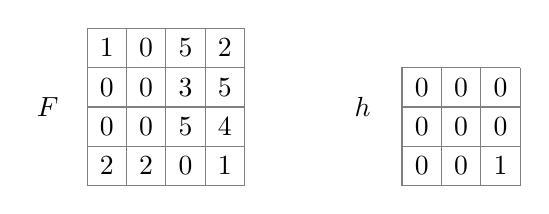
\begin{tikzpicture}
\node at (-1.5, 0) {$\mb{F}$};
\draw[step=0.5cm, color=gray] (-1, -1) grid (1, 1);
\node at (-0.75, +0.75) {1};
\node at (-0.25, +0.75) {0};
\node at (+0.25, +0.75) {5};
\node at (+0.75, +0.75) {2};
\node at (-0.75, +0.25) {0};
\node at (-0.25, +0.25) {0};
\node at (+0.25, +0.25) {3};
\node at (+0.75, +0.25) {5};
\node at (-0.75, -0.25) {0};
\node at (-0.25, -0.25) {0};
\node at (+0.25, -0.25) {5};
\node at (+0.75, -0.25) {4};
\node at (-0.75, -0.75) {2};
\node at (-0.25, -0.75) {2};
\node at (+0.25, -0.75) {0};
\node at (+0.75, -0.75) {1};

\node at (2.5, 0) {$\mb{h}$};
\draw[step=0.5cm, color=gray] (2.99, -1) grid (4.5, 0.5);
\node at (3.25, +0.25) {0};
\node at (3.75, +0.25) {0};
\node at (4.25, +0.25) {0};
\node at (3.25, -0.25) {0};
\node at (3.75, -0.25) {0};
\node at (4.25, -0.25) {0};
\node at (3.25, -0.75) {0};
\node at (3.75, -0.75) {0};
\node at (4.25, -0.75) {1};
\end{tikzpicture}

\begin{solution}[0.75in]
{\color{red} TBA}
\end{solution}
\end{blocksection}

%%%

\begin{blocksection}
\question Match the images to the descriptions.

\begin{figure}[H]
\includegraphics[width=0.75\textwidth]{airplane}
\end{figure}

\begin{solution}[0.75in]
{\color{red} TBA}
\end{solution}
\end{blocksection}

%%%

\begin{blocksection}
\question One application of filtering/convolution is template matching: finding regions in an image that are similar to a given patch. How would you imagine that this is done?

\begin{solution}[0.75in]
{\color{red} TBA}
\end{solution}
\end{blocksection}

%%%

\begin{blocksection}
\question Give a $3 \times 3$ linear filter that shifts an image one pixel to the right and increases the image brightness by 50\%.

\begin{solution}[0.75in]
{\color{red} TBA}
\end{solution}
\end{blocksection}

%%%

\begin{blocksection}
\question How do you obtain an edge image if you're only allowed a blurring filter?

\begin{solution}[0.75in]
{\color{red} TBA}
\end{solution}
\end{blocksection}
